\chapter{WfSteer: An Approach for Managing User Steering Action Data} \label{chap4}

We informally defined steering actions as interactions that the user performs during workflow steering, like online data analysis and online data adaptation, in Section \ref{chap2_sec_basic_concepts} and presented formal definitions on the dataflow-oriented approach in Section \ref{subsec_datacentric}.
Here in this chapter, we introduce WfSteer, our approach for managing user steering action data in large-scale workflows.
We begin by motivating the need for management of a new type of data, steering action data, to support steering in CSE (Sec \ref{sec_steering_action_data}).
Then, we extend the dataflow-oriented approach to formally define \textit{user steering action} and \textit{steering action data} 
(Sec. \ref{user_steering_def}) and define instances of steering actions following these definitions
(Sec. \ref{sec_online_data_adaptations}). 
Finally, in Section \ref{sec_provdfa} we introduce the notion of provenance of steering actions  and present a new W3C PROV-compliant data diagram to model it.
The conceptual parts that encompass the two typical ways of conducting CSE experiments on large-scale computers (\ie{} workflow scripts and WMSs) have been unified here in this chapter.
Then, in Chapters \ref{chap_dfadapter} and \ref{chap_dchiron}, we introduce the specific details on how WfSteer is instantiated to manage steering action data in workflow scripts and in a WMS, respectively.



\section{User Steering Action Data: a new type of data that needs to be managed}
\label{sec_steering_action_data}

After users have analyzed partial data and gained insights,
they may decide to adapt the workflow execution online.
In this thesis, an \textit{online data adaptation}, or adaptation for short,
is a steering action performed by a user that causes a change
in the flowing data elements in the dataflow.
Adaptations bring powerful abilities to users, putting the human in control of a scientific workflow execution.
They can significantly reduce overall execution time, since users are able to identify a satisfactory result before the programmed number of iterations.
The adaptable aspects range from computing resources involved in the execution (\eg{} adding or removing nodes), to check-pointing and rolling-back, reducing datasets, tuning of filter thresholds, loop-stop conditions, and parameter values.

Populating a workflow database (Sec. \ref{subsec_wfdb}) during workflow execution enables both online data analysis and adaptation.
For example, it is possible to analyze or monitor the data being continuously generated as the workflow executes \cite{Silva2017Raw},
change filter conditions during execution \cite{Dias2011Supporting},
and adapt loop conditions of iterative workflows (\eg{} modify number of iterations or loop stop conditions)
\cite{Dias2015Data-centric}.

In a long-running execution, many interactive data analysis and
adaptations may occur.
When a user adapts the dataflow, new data type of data, \textit{steering action data}, are generated and, hence, must be managed,
\ie{} captured, related and stored in a database, integrated with the rest of the workflow data (\ie{} execution, domain, and provenance).
Since provenance data are so beneficial, we consider that when a user
interacts with the workflow execution, the provenance of the generated steering action data must be stored in a database as well.
By bot doing so, users can easily lose track of what and how they
have steered in the past, negatively impacting results reliability, validation, and
reproducibility.
For example, if a user removes subsets of a dataset (data reduction-kind of adaptation),
the tasks (execution data) that would consume them will not need to be
executed, leading to inconsistencies or spending unnecessary time if the tasks are executed \cite{Souza2017Data}.
In another example, if a user fine-tunes parameters of a program, the overall result may be
changed.

Furthermore, enriching the workflow database steering action data,
jointly with provenance, execution, and domain data, enables future interaction
analysis. In addition to reliability and reproducibility, having such
data enables users to learn from their own adaptations: they may find
that when they tune certain parameters to a given range of values, the
convergence of the solver improves by a certain amount. Finally, these
steering action data allow for building \myabbrev{AI}{Artificial Intelligence}-based systems that help users
while they are steering simulations \cite{Silva2018JobPruner:},
as they can extend their training database with provenance of
adaptations. Thus, the computational steering systems, including WMSs with steering support, should
manage steering action data, which has never been done before.


\section{User Steering Action and Data Definitions}
\label{user_steering_def}

As defined in Definition \ref{def:dataflow}, a dataflow $Df$ is represented as $Df = (T,D,\Phi)$. Given this, we define User Steering Action as follows.

\begin{mydef}{def:steeringaction}{User Steering Action}
A user steering action $SA$ is an interaction between a user who analyzes or monitors or dynamically adapts one or more elements of $DS$:
$$DS' \leftarrow SA_\alpha(DS)$$
where $DS \in D$ is a dataset in the dataflow that the user can steer, $\alpha$ is a steering action clause that delimits the scope of the steering action resulting in $DS'$.
\end{mydef}

For instance, in a parameter sweep workflow steered by a user, an input dataset $I_{DS}$ can have its composing data elements dynamically adapted by the user. In this case, $\alpha$ contains the criteria to specify which elements would be affected by the action, resulting in the dynamically modified dataset $I_{DS}'$. This example is explored in the next section.

To allow for tracking a user steering action $SA$, steering action data need to be managed, \ie{} captured, related to the rest of the workflow data, and stored in a database ready for online data analysis.
User steering data consist of data informing:
\textit{when} the action happened,
\textit{why} the user decided to act,
\textit{how} the action occurred,
\textit{which} workflow data were analyzed or adapted,
\textit{what} was happening before and after the action,
\textit{who} acted, and
the type of the action itself (\eg{} parameter tuning, data reduction, query).

\begin{mydef}{def:usersteeringdata}{User Steering Action Data}
User Steering Action Data $SD$ are important information that helps to understand the steering actions and their influence on the workflow data.
User Steering Action Data $SD$ are represented as:
$$SD = (
DS,
DS',
\alpha,
U,
\Gamma,
\mu,
\psi
)$$
where:
\begin{itemize}
    \setlength\itemsep{-2mm}
    \item[-] \noindent
        $DS$, $DS'$ and $\alpha$ are the datasets and the clause, respectively, involved in the action $SA$;
    \item[-] \noindent
        $U$ contains data about the user who performed $SA$;
    \item[-] \noindent
        $\Gamma$ is a set of data transformation executions (tasks) related to SA;
    \item[-] \noindent
        $\mu$ contains metadata of the steering action $SA$ itself, such as the type of the action, wall time during which the action lasted, descriptions informed by the user at the moment of the action; and
    \item[-] \noindent
        $\psi$ is an optional argument representing any other data, in the same context of the steering action $SA$, which can benefit the register of the steering action.
\end{itemize}

\end{mydef}

\section{Definitions for Online Data Adaptations} \label{sec_online_data_adaptations}


Adaptations have a characteristic of either update (we call them \textit{U-adaptation}), or insert or delete (called \textit{I/D-adaptation}).
U-adaptations are steering actions that update data values, like adjustments, fine-tunings, or any modification of one or more data elements in the dataflow. Parameter tuning is an example of U-adaptations.
I/D-adaptations are steering actions that cause addition or deletion of data elements in the dataflow. Data reduction is an example of I/D adaptations. In this section, we define these two examples of adaptations as special cases of the Steering Action general Definition \ref{def:steeringaction}.

\begin{mydef}{def:tune}{Tune}
$Tune$ is a steering action for tuning parameters, represented as follows:
$$I'_{DS} \leftarrow Tune_{(\eta,C)}(I_{DS})$$
where:
\begin{itemize}
    \setlength\itemsep{-2mm}
    \item[-] \noindent
         $I_{DS}$ contains old values of attributes being tuned into $I'_{DS}$ with the new values.
         $I'_{DS}$ follows the same schema $\mathbb{S}(I_{DS})$ and semantics $\Sigma(I_{DS})$ of the input dataset $I_{DS}$;
    \item[-] \noindent
        $(\eta,C)$ is the steering action clause;
    \item[-] \noindent
        $\eta$ is a set of ordered pairs $(p,v)$, where $p \in P_I \subset \Sigma(I_{DS})$ is the parameter being tuned and $v$ is its new value;  and
    \item[-] \noindent
        $C$ expresses a predicate to address a specific data element that is having its parameters tuned. In case of an $I_{DS}$ that contains a single data element, $C$ is optional.
\end{itemize}

To register a $Tune$ action, the steering action data $SD_{Tune}$ managed are:
$$SD_{Tune} = (
I_{DS},
I'_{DS},
(\eta,C),
U,
\Gamma,
\mu,
\psi
)$$
\end{mydef}


\begin{mydef}{def:cut}{Cut}
$Cut$ is a steering action for data reduction. It cuts data elements of an input dataset $I_{DS}$. It is represented as follows:
$$I'_{DS} \leftarrow Cut_{C}(I_{DS})$$
where:
\begin{itemize}
    \setlength\itemsep{-2mm}
    \item[-] \noindent
        $I_{DS}$ is the input dataset that is having its data elements being removed by the cut, resulting into $I'_{DS}$, s.t. $|I'_{DS}| < |I_{DS}|$, which is the new dataset after the cut.
        $I'_{DS}$ follows the same schema $\mathbb{S}(I_{DS})$ and semantics $\Sigma(I_{DS})$ of the input dataset $I_{DS}$ ;
    \item[-] \noindent
        $C$ is the criteria that addresses the slice of input data elements that are removed. $C$ may either be a simple predicate (\eg{} $a_1 = FATIGUE$) or a min-term predicate (\eg{} $a_2 > 38 \wedge a_3 > 0.1$).
\end{itemize}

To register a $Cut$ action, the steering action data $SD_{Cut}$ managed are:
$$SD_{Cut} = (
I_{DS},
I'_{DS},
C,
U,
\Gamma,
\mu,
\psi
).$$
\end{mydef}




\section{Modeling Steering Action Data using W3C PROV Concepts}
\label{sec_provdfa}

In Section \ref{sub_w3cprov}, we discussed W3C PROV and its specializations for
workflows, like PROV-Wf \cite{Costa2013Capturing} and ProvONE \cite{ProvONE}.
\citet{Silva2017Raw} have modeled the dataflow concepts presented in
Section \ref{subsec_datacentric} using another PROV specialization, called
PROV-Df.
In this thesis,
instead of creating a completely new provenance model, we first begin by
consolidating a base model using several past contributions to the W3C-compliant provenance data diagrams PROV-Wf and
PROV-Df \cite{Souza2017Data, DeOliveira2015How, Silva2017Raw, Costa2013Capturing} to introduce a W3C PROV-compliant provenance data diagram that specializes PROV concepts to model user steering actions. We call it \textit{PROV-DfA}.
By adhering to the well-established W3C PROV standard,
our approach aims at allowing for interoperability among
other provenance databases.
In addition, another important principle is that the W3C PROV and its extensions PROV-Wf and PROV-Df are abstract and flexible
enough to be used in different domains or applications, such as Astronomy, Bioinformatics, and O\&G \cite{Ocana2011SciPhy:,Silva2017Raw,Souza2017Data,Costa2013Capturing}. A general overview of PROV-DfA using an UML class diagram is illustrated in Figure \ref{fig:prov_dfa_dataschema}.  
For the sake of comprehension of the figure, we only show the classes and their relationships. The relevant classes' attributes are not shown in the figure, but discussed in the text. 

\begin{figure}[H]
    \centering
    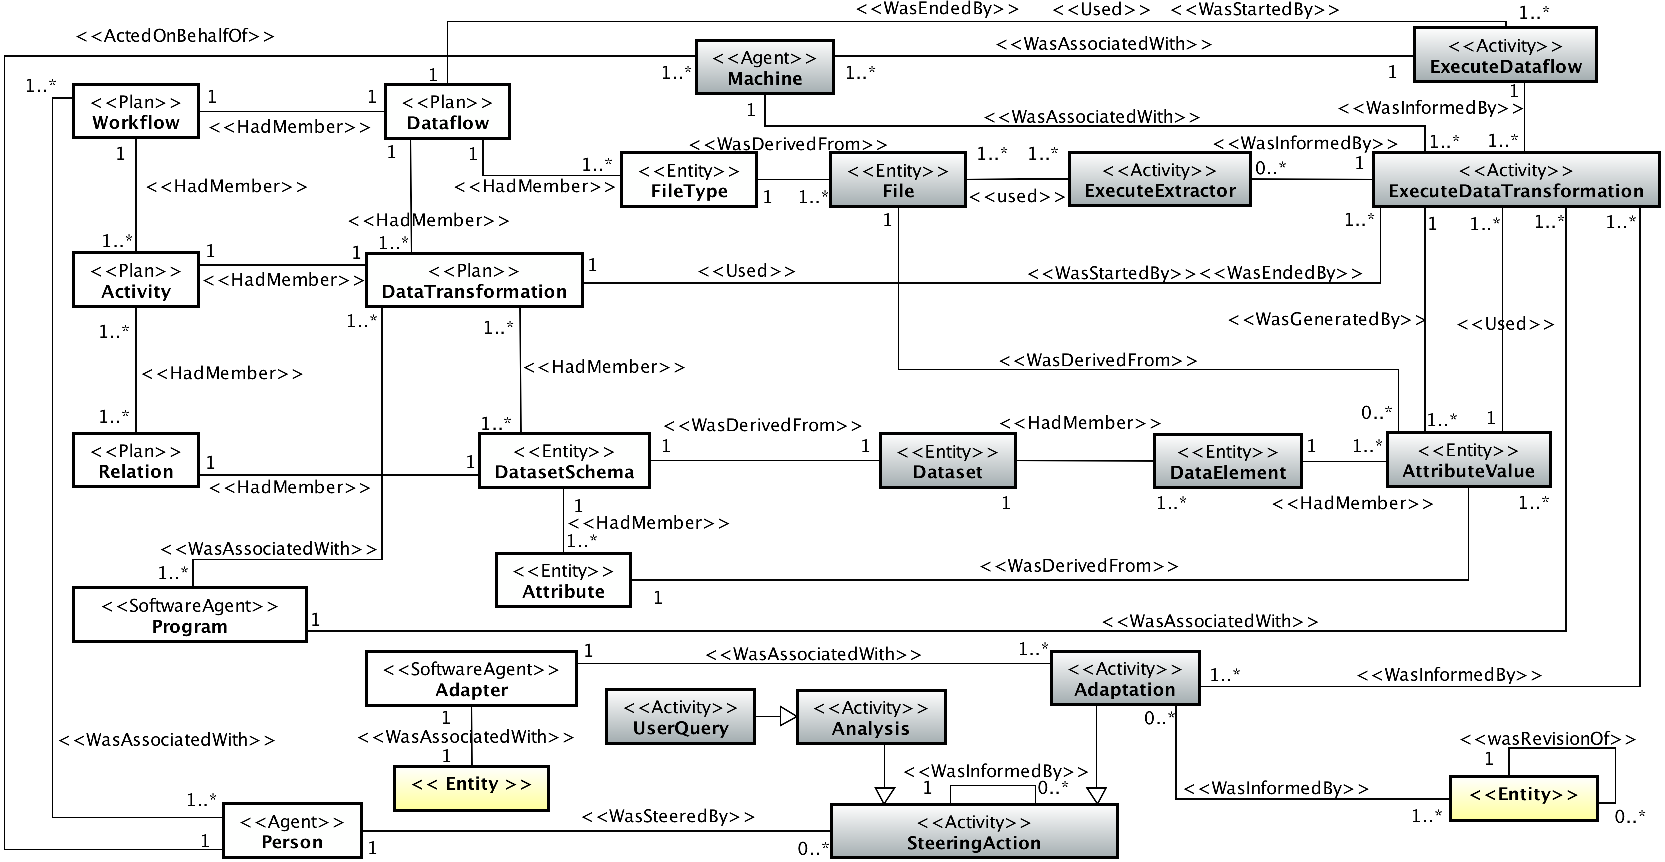
\includegraphics[width=\textwidth]{img/PROV-DfA.png}
    \caption{PROV-DfA overview. A larger visualization is on GitHub \cite{PROV-DfA_GitHub}.}
    \label{fig:prov_dfa_dataschema}
\end{figure}




\subsubsection{PROV-DfA's General Concepts}
\label{sec:prov_dfa_general_concepts}


We use \codefont{prov:} namespace to indicate the PROV classes or relationships.
Each \codefont{ExecuteDataTransformation} consumes (\codefont{prov:used}) and produces
(\codefont{prov:wasGeneratedBy}) \codefont{AttributeValues}.
These values may have been extracted by an \codefont{ExecuteExtractor} \cite{Silva2017Raw}.
Data elements compose the dataset (\codefont{Dataset}).
For prospective provenance, the dataset has an associated \codefont{DatasetSchema},
which is composed of \codefont{Attribute}.
\codefont{Attributes}
describe the
\codefont{AttributeValues} generated during execution.
They have a data type (\eg{} integer, text) and may have extra fields in the
\codefont{Attribute} class to allow for attribute specification (\eg{} determine if the
attribute semantics is in
$\{F_{I}, F_O, V_I, V_O, P_I, L_I, L_O, C_O\}$ --- Def. \ref{def:semantics_attributes}).
Data about execution, such as task's (\ie{} data transformation execution)
wall time and performance data (CPU, memory), linkage to subsequent and previous
tasks, and their related prospective and retrospective provenance can be stored
relating to instances of \codefont{ExecuteDataTransformation}.

Next, PROV-DfA adds specialized classes and relationships to represent steering actions
and steering action data.
PROV-DfA introduces the classes \codefont{SteeringAction},
\codefont{Analysis},
\codefont{Adaptation},
and
\codefont{Adapter};
and the relationship
\codefont{WasSteeredBy}.
We use a UML class diagram, where the \codefont{<<stereotypes>>} in classes specify
PROV superclasses (mainly \codefont{Agents}, \codefont{Entities}, and \codefont{Activities}); and the
\codefont{<<stereotypes>>} between classes specify relationships.
Classes in white background represent prospective provenance, whereas in gray
represent retrospective provenance. \codefont{prov:Entity} in yellow means that classes
in PROV-DfA that are subclasses of \codefont{prov:Entity} (prospective or retrospective)
can be used in place, as explained next.


In PROV-DfA, adaptation is represented by \codefont{Adaptation}, a subclass of
\codefont{Steering Action}, subclass of \codefont{prov:Activity}.
An adaptation was steered by
(\codefont{wasSteeredBy}) a \codefont{prov:Person},
occurred at a specified time (class attribute \codefont{prov:startedAtTime}),
had an adaptation characteristic (class attribute \codefont{adaptationCharacteristic}) that can be
``update'' or ``insert/delete'', in case of U-adaptations or I/D-adaptations,
respectively.
Users may add a description to the adaptation to describe, \eg{} what was going
on in the experiment when they decided to perform a specific change.
Also, as inherited by \codefont{SteeringAction}, an \codefont{Adaptation} may have been
informed by another \codefont{Adaptation}, hence the auto-relationship \codefont{prov:wasInformedBy}.
This is the case, for example, of a rollback adaptation, requested by a user,
that happened right after the user modified parameters in a simulation,
which is another adaptation.

Since adaptations in the dataflow occur while the workflow is executing,
it is important to manage the execution state data.
The most representative PROV-DfA activity that represents the execution state is \codefont{ExecuteDataTransformation}.
When an adaption occurs, these instances carry information about time,
pointers to domain data being consumed or produced,
and computational resources being consumed.
Thus, being able to track which specific data transformation was running
at the moment of the adaptation may be very useful for analyses that integrates
adaptation with provenance, domain, and execution data.
For this, we relate which \codefont{ExecuteDataTransformation} instances were influenced
(\codefont{prov:wasInformedBy}) by adaptations.
How adaptations relate to \codefont{ExecuteDataTransformation}, as well as how
\codefont{prov:Entities} are affected depend on characteristic of the online adaptation,
as explained next.

\textit{Adapter} is a software service (it can be implemented, \eg{} as a function in a workflow script or a method in the WMSs code)
that knows the communication protocol
capable of adapting the running workflow following the command issued by the user. That is, it knows how to adapt the elements of the
dataflow in a running workflow. Since it is a software service,
it is a subclass of \codefont{prov:SoftwareAgent}.
When the user decides to adapt an element of the dataflow, the Adapter
is responsible for modifying the requested element.
Any information that describes the Adapter (\eg{}
which element of the dataflow it adapts,
where the program can be located in the file system,
how it can be invoked) may be stored relating to the \codefont{Adapter} class.
Adapter relates to classes that are subclasses of \codefont{prov:Entity} and to the
adaptation itself (via \codefont{prov:wasAssociatedWith}).

When the user performs a U-adaptation, a new instance of \codefont{Adaptation} is created.
Also, a new instance of one of the \codefont{prov:Entity} subclasses in PROV-Df is created
(\eg{} \codefont{AttributeValue}, \codefont{DataTransformation}) containing the new data,
which will replace the old data in the dataflow.
The newly created entity is related (\codefont{prov:wasInformedBy}) to the adaptation.
Moreover, the newly created data is related to the old one via
\codefont{prov:wasRevisionOf}, so that the association between the new and old data is maintained.
Additionally, to relate the adaptation with execution state, PROV-DfA relates
(\codefont{prov:wasInformedBy}) the
\codefont{ExecuteDataTransformation} instances that were in ``running''
state at the moment of the adaptation.
Finally, \codefont{Adapter} is related to the prospective entity (\eg{} \codefont{Attribute}, \codefont{DataTransformation})
that specifies the entity adapted.

When the user performs an I/D-adaptation, a new instance of \codefont{Adaptation} is created and there is a relationship (\codefont{prov:wasInformedBy}) between the \codefont{Adaptation} and the added or deleted instances of a \codefont{prov:Entity} subclass.
In case of deletions, the entity is not physically deleted from the workflow database,
for the sake of provenance.
Rather, it is assumed that when an \codefont{Adaptation} is a deletion,
the deleted instance is logically deleted from the dataflow. This enables tracking entities deleted online. Since adding or deleting elements affects the execution, the instances of ExecuteDataTransformation directly affected by the added or deleted elements of the dataflow are related (\codefont{prov:wasInformedBy}) to the \codefont{Adaptation} instance.
For example, in a data reduction, data transformations that are supposed to execute are not executed because of a adaptation.
These not executed instances of \codefont{ExecuteDataTransformation} are related to the \codefont{Adaptation} instance. Finally, \codefont{Adapter} and \codefont{Adaptation} are related similarly as in U-adaptations.

In summary, in PROV-DfA, an \codefont{Adaptation} is a \codefont{prov:Activity} steered by a \codefont{prov:Person}, which influenced instances of classes that are subclasses of
\codefont{prov:Entity}, and influenced instances of \codefont{ExecuteDataTransformation}.
The
\codefont{Adapter} software relates to the prospective entity being adapted and to the adaptation.

\subsubsection{Modeling Specific Steering Actions using PROV-DfA}

In this section, we specialize PROV-DfA concepts to represent online parameter tuning, changes in loop control, and data reduction as PROV-DfA's \textit{U} and \textit{I/D-adaptations}.


\subsubsubsection{Parameter Tuning}

Parameter tuning refers to the action of steering parameters of a data transformation in a dataflow, like numerical solver parameters or machine learning model hyperparameters. In PROV-DfA, ParameterTuning is a specialization of Adaptation. Parameter tunings are adaptations in attribute values (AttributeValue) that are related to data elements (\codefont{DataElement}) related to $I_{DS}$ (\codefont{Dataset}) of a certain data transformation (\codefont{DataTransformation}).
The attribute value modified must have been derived from (\codefont{prov:wasDerivedFrom})
an \codefont{Attribute} whose attribute specification is $P_I$.
As a U-adaptation, a new instance of \codefont{ParameterTuning} is created and related to the new instance of its adapted entity, \ie{} \codefont{AttributeValue}, with the new value for the parameter.
The new value is related to the old one via \codefont{prov:wasRevisionOf}.
\codefont{ExecuteDataTransformation} instances running at the moment of the adaptation are related to the \codefont{Adaptation} instance.
Finally, since users tune parameters of data transformations, the \codefont{Adapter} relates to the \codefont{DataTransformation} associated to \codefont{DatasetSchema} that had the \codefont{Attribute} modified.

\subsubsubsection{Online Adaptation of Iterative Simulations}

Workflows with an iterative workflow execution model have data transformations that evaluate loops. Using the dataflow-oriented approach concepts, values for these loop-stop conditions are
modeled as an attribute in $L_I$ of a data transformation that evaluates a loop and the iteration counter is modeled as an attribute in $L_O$ of the data transformation.
Moreover, each iteration generates an instance in \codefont{ExecuteDataTransformation} for the loop evaluation. During execution of each iteration, a relationship between the output of this data transformation, containing the current iteration value, and the \codefont{ExecuteDataTransformation} instance is particularly useful for such workflows, as it identifies a specific part of the workflow execution, and often users can analyze results as the workflow iterates.
Such control information is important for the adaptation, as users can associate their specific actions with execution data, such as which point in workflow elapsed time that action happened or what memory or CPU consumption were.

In PROV-DfA, such adaptations are represented as \codefont{LoopAdaptation}, a subclass of \codefont{Adaptation}.
Similarly to \codefont{ParameterTuning}, its instance is related to the new instance of \codefont{AtrributeValue}, containing the new value for the loop control condition, relating (\codefont{prov:wasRevisionOf})
to the old one.
The adapted instance of \codefont{AttributeValue} must be derived from an \codefont{Attribute} whose attribute semantics is $L_I$.
Additionally, the generated \codefont{ExecuteDataTransformation} instance related to the output of the last iteration (\ie{} last execution of the data transformation for loop evaluation) is related to the \codefont{LoopAdaptation} instance.
Finally, the adapter must be able to dynamically modify the data transformation that represents the loop evaluation. That is, \codefont{Adapter} in this case relates to \codefont{DataTransformation}.


\subsubsubsection{Data Reduction}

Online user-steered data reduction is very useful for reducing execution time and amount of data to be processed during a simulation \cite{Souza2017Data}.
\codefont{DataReduction} is a subclass of \codefont{Adaptation}.
In the dataflow-oriented approach, data files are represented as pointers in $F_I$,
whereas $V_I$ contain extracted domain values from those files specified in $F_I$.
An approach to reduce data is to specify a criteria based on $V_I$ values to eliminate files
in $F_I$ to be processed, enabling the adapter program to logically delete data elements in  $I_{DS}$. This makes the application not to execute the data transformations for the removed elements.
Analogously, in PROV-DfA, reducing data means to logically remove instances of \codefont{DataElement} (and consequently \codefont{AttributeValues}) of a \codefont{Dataset} ($I_{DS}$).
This can be the result of an I/D adaptation.
Thus, there is a relationship (\codefont{prov:wasInformedBy}) between the removed instances of \codefont{DataElement}
and \codefont{AttributeValue} and the adaptation. The \codefont{ExecuteDataTransformation} instances that would use (\codefont{prov:used}) the removed \codefont{AttributeValue} instances are related to the \codefont{DataReduction} instance. Additionally, the criteria to remove data elements is stored within the adaptation instance.
Finally, as users remove data elements in $I_{DS}$, the adapter is related to the \codefont{DataTransformation} associated to the \codefont{Dataset} that had the \codefont{DataElement} and \codefont{AttributeValues} removed.


\subsubsubsection{Applying the Dataflow-oriented Approach with PROV-DfA}

Now we apply the concepts defined in Sections \ref{subsec_datacentric} and \ref{user_steering_def}
to put the PROV-DfA provenance data diagram into practice to illustrate with a concrete example of its use in the libMesh-sedimentation workflow.

In Figure \ref{fig:libmesh_with_provdfa}, we show large raw input files (with mesh data) stored on disk,
with pointers in the solver's input dataset $I_{DS}$.
$I_{DS}$ has over 70 parameters, among which only two are displayed in the figure
(flow linear and non-linear tolerance).
These solver parameters are extracted from a configurations file, which is
read at each iteration.
Yet, the maximum number of iterations ($t_{max}$) is a $L_I$ attribute of the
data transformation solver.
Metadata are extracted ($V_I$) from input raw files at runtime to allow for tracking
their contents while they are processed.
Elements of $O_{DS}$ of each data transformation are also collected
(via raw data extractors and source code instrumentation) and stored in the database.
For example, the solver $O_{DS}$ contains calculated values,
such as linear and non-linear results, as well as the current time iteration value.
In addition to online data analyses, the user performs several adaptations during the simulation.

\begin{figure}[H]
    \centering
    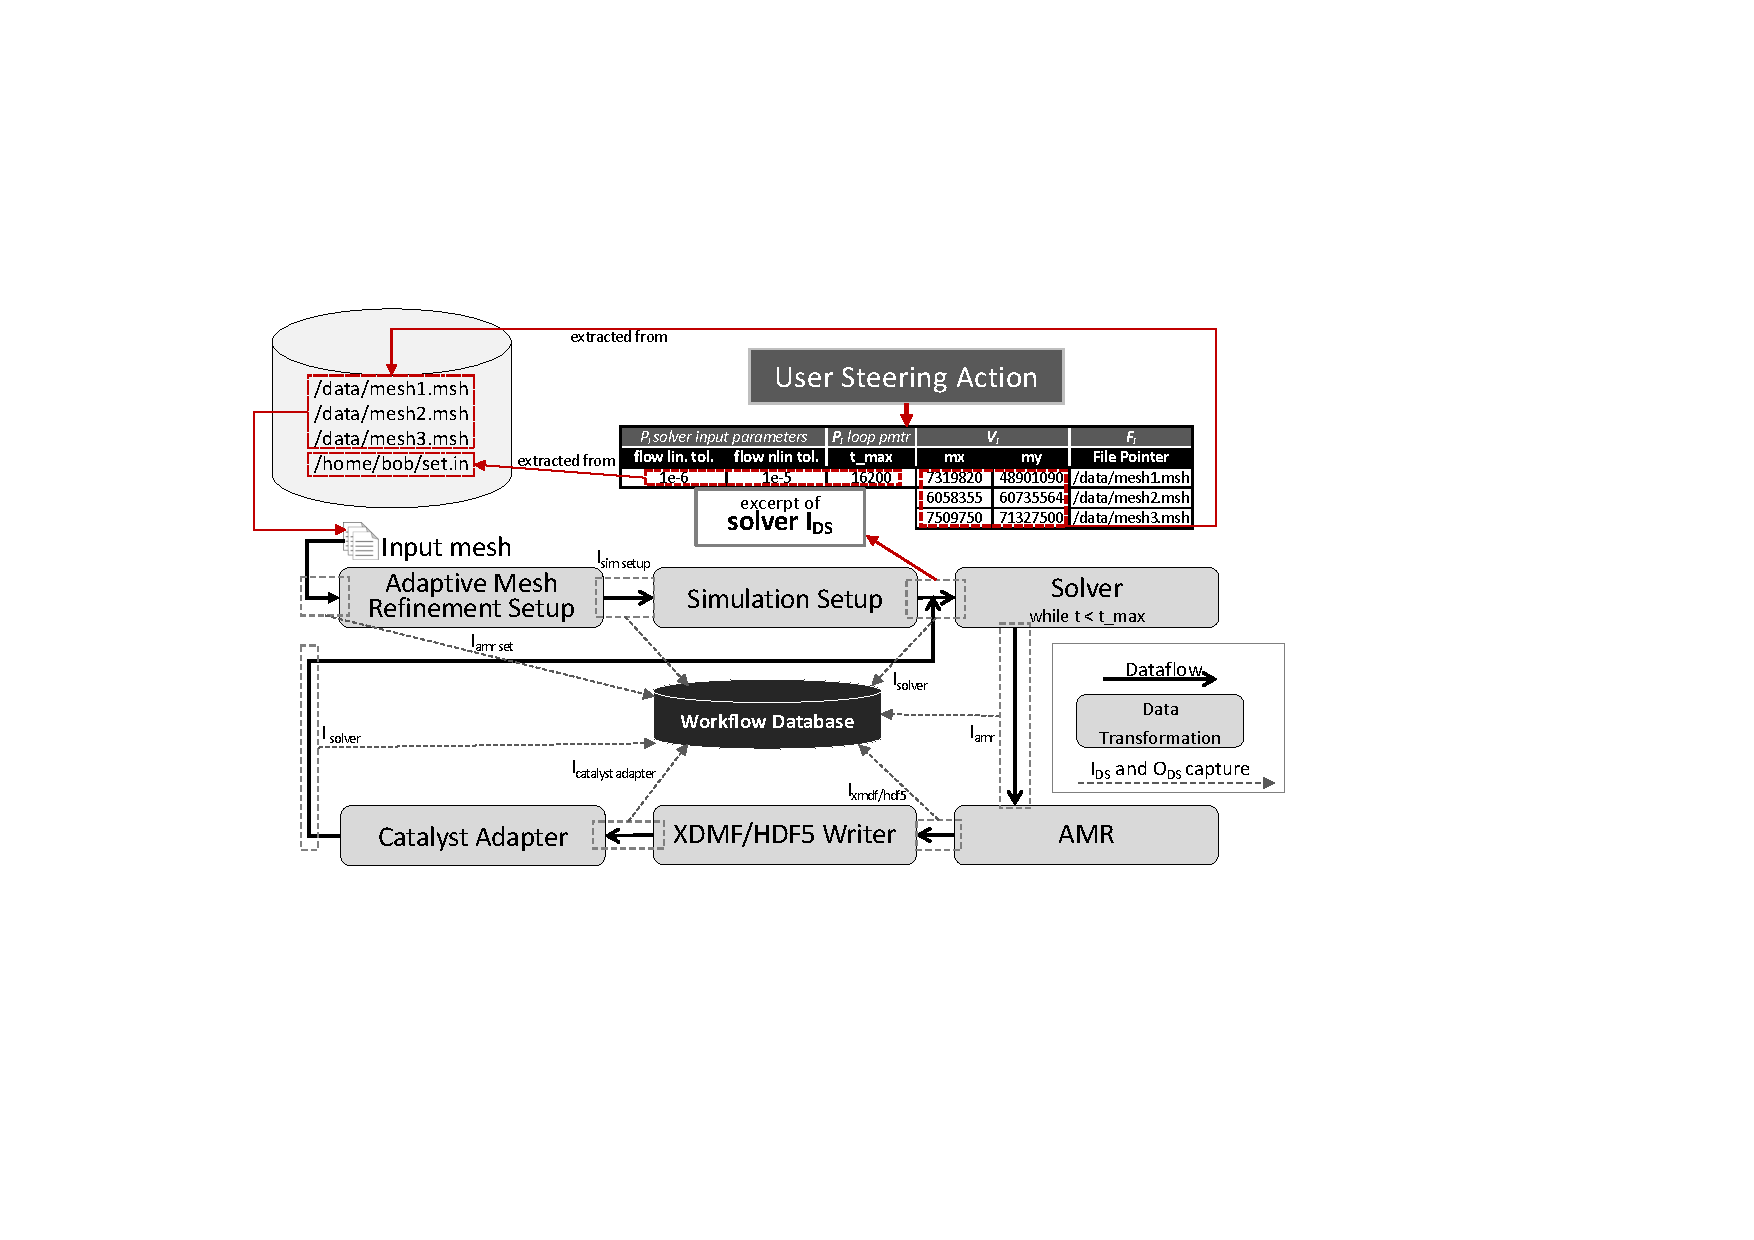
\includegraphics[width=\textwidth,keepaspectratio]{img/steeringaction-provdfa.pdf}
    \caption{Dataflow in the libMesh-sedmentation simulation using the dataflow-oriented approach with PROV-DfA.}
    \label{fig:libmesh_with_provdfa}
\end{figure}

In Figure \ref{fig:visualization_using_provdfa},
we present a visualization of an excerpt of the data in a workflow database
implementing PROV-DfA.
It shows a user tuning the flow linear tolerance parameter from $\num{1e-5}$ to
$\num{1e-3}$ and a data reduction with criteria $mx < \num{7e6}$.


\begin{figure}
    \centering
    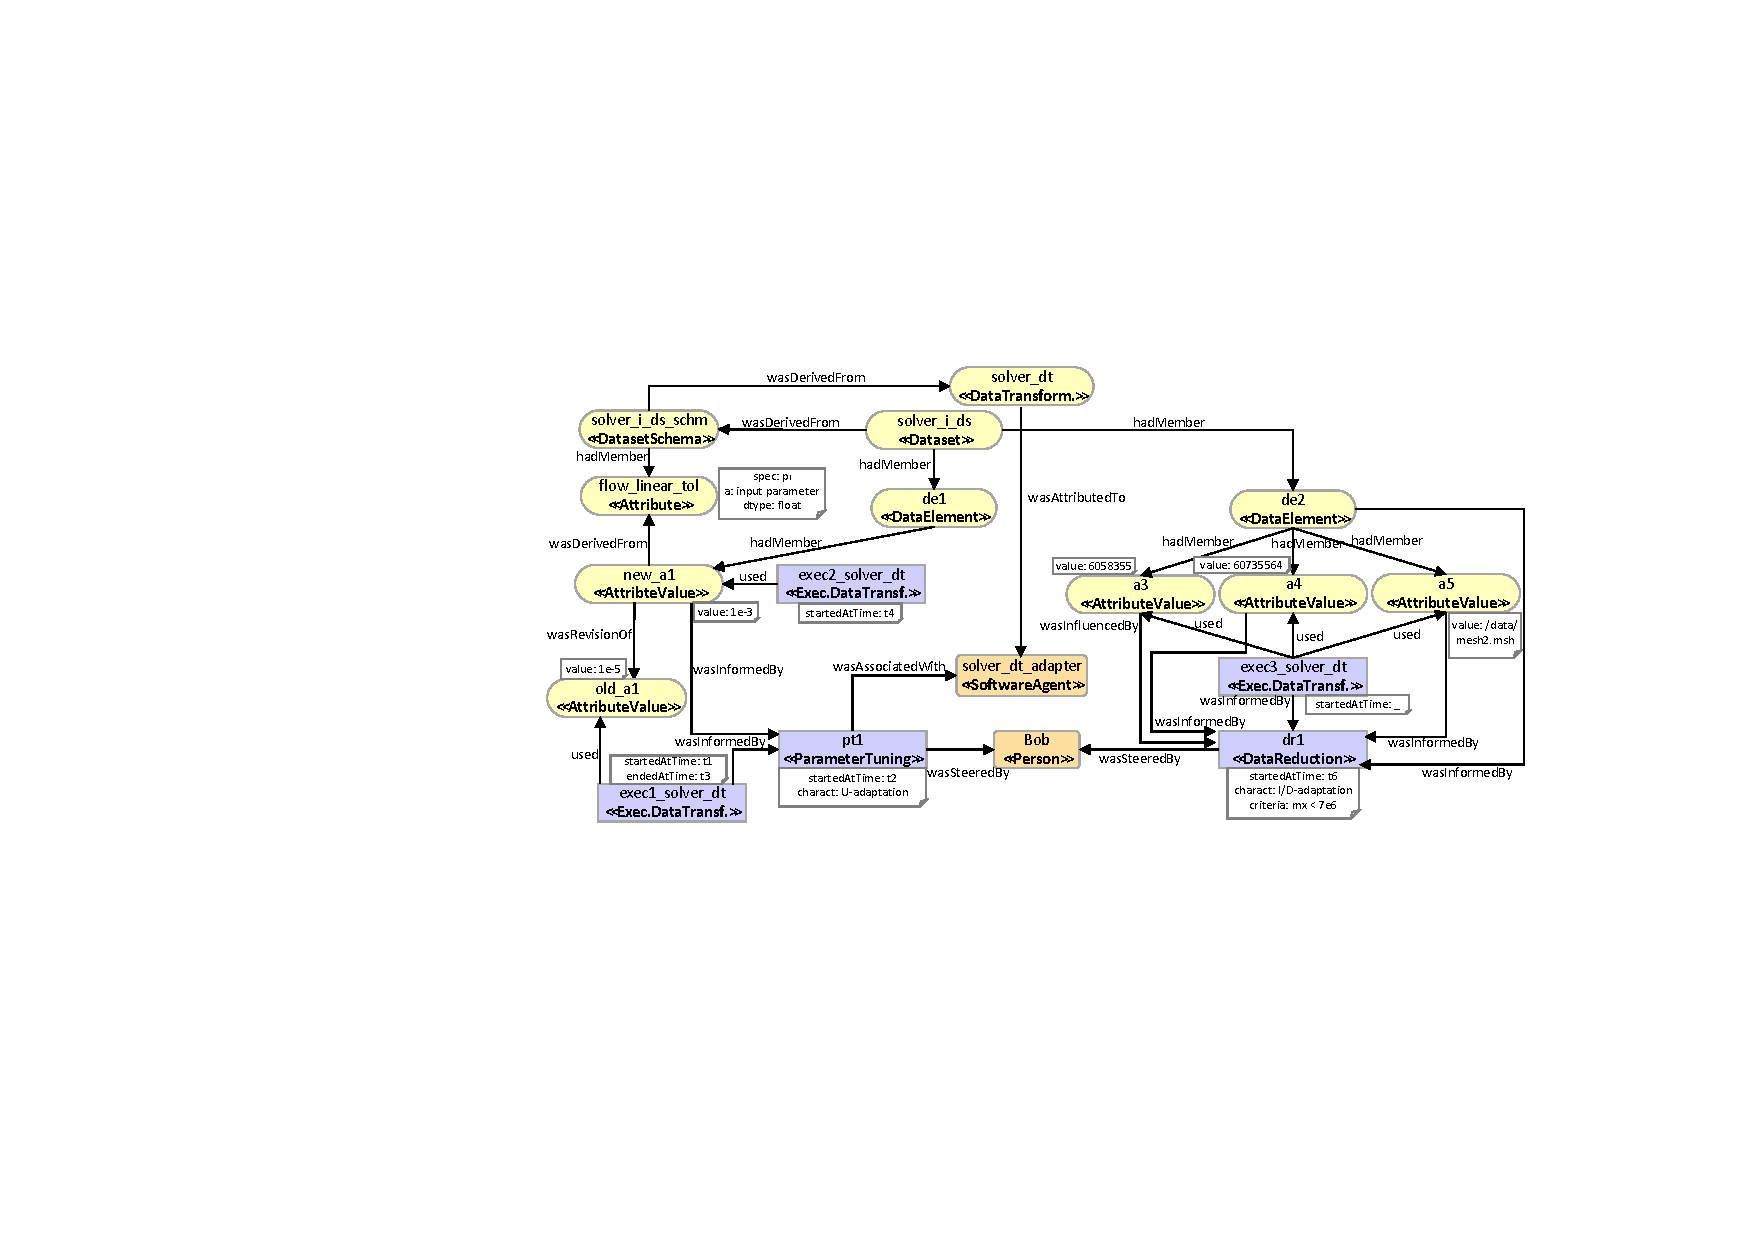
\includegraphics[width=\textwidth,keepaspectratio]{img/PROV-DFA-EXAMPLE.pdf}
    \caption{Visualization of data using PROV-DfA.}
    \label{fig:visualization_using_provdfa}
\end{figure}


By using data in a relational workflow database implementing PROV-DfA,
users can run the following queries (their SQL codes are on GitHub \cite{PROV-DfA_GitHub}).


\begin{itemize}
    \setlength\itemsep{-2mm}
    \item[-] \noindent
    \textit{Inspecting parameter tunings (``who", ``when", ``what")}

    How many tunings did the user do? Which parameters did the user change?
    What were the values when the user changed and what values did the user change into?
    When did each adaptation happen?

    \item[-] \noindent
    \textit{Inspecting parameter tunings (``how")}

    In parameter tuning 3, how was the main solver output values 10 iterations before and after?

    \item[-] \noindent
    \textit{Data reduction (``how", ``which")}

    On average, how long iterations were lasting before and after the user
    reduced input files from the input data? Which files were affected?

\end{itemize}

These queries show the potential of PROV-DfA for workflow databases allowing for tracking user steering action data in large-scale workflows.





\section{Adaptive Monitoring Concepts}
\label{sec_adaptive_monitoring_concepts}

In this section, we present an adaptive monitoring approach that
combines monitoring and adaptation. 
It helps users following the
evolution of the workflow data being generated during execution, interesting parameters, QoIs, and result data. Since what
users find interesting may change over time, this approach allows the
user to adapt the monitoring definitions, such as which data should be
monitored and how.
The adaptive monitoring relies on online queries to
the continuously populated workflow database. Users can set up
queries (such as the ones in Tables \ref{tab:queries1} and \ref{tab:queries2}) to monitor the data, analyze monitoring results, and
adapt monitoring settings.

Monitoring works as follows. There is a query set $QS$ composed of
monitoring queries $q_i$, 
$0 \leq i \leq |QS|$,
each one to be
executed at each $\Delta t_i > 0$ time intervals. Users do not need to
specify queries at the beginning of the execution, since they do not know
everything they want to monitor. This is why $QS$ starts empty.

After users gain insights from the data, after interactive 
data analyses, they can add monitoring queries to $QS$ in an
\textit{ad-hoc} manner. 
Each $\Delta t_i$ can be adapted, meaning that users
have control of the time frame of each $q_i$ during
execution. The monitoring queries and settings are stored in the
workflow database.

Each $q_i$ execution generates a monitoring query result set $qr_{it}$, $t = \{k\Delta t_i | k \in \mathbb{N}_{\geq 0}\}$, at each
time interval $\Delta t_i$. This result set is also stored in the
workflow database.
The users have the flexibility to adapt the monitoring during
workflow execution. To do so, at each time instant $t$ after each
monitoring query result $qr_{it}$ has been generated,
the values for $\Delta t_i$ and $q_i$ are reloaded from the
workflow database. If any change has happened, it will be considered in the
next iteration $t + \Delta t_i$.
Moreover, at each certain time during
execution (also configured by the user), there is a check to verify if the user
has added new monitoring queries in $QS$. This approach takes 
advantage of the data stored online in the workflow database to enable users
to adapt monitoring settings, including which data will be monitored and
how.




In the next chapter, we present the first instantiation of WfSteer to support workflow scripts.